\chapter{The Economics of Migration: The Migrant}

\fancyhead[L]{ECON0024}
\fancyhead[C]{Ch.11 The Economics of Migration: The Migrant}
\fancyhead[R]{Kuangjie Ni}
\fancyfoot[L]{\hyperlink{tableofcontents}{Back to Table of Contents}}
\fancyfoot[R]{Kuangjie Ni}

\section{Intro: Motivation}
\begin{itemize}
    \item \emphb{Definition of Migration}: movement of individuals from one region to another
    \begin{itemize}
    \item International migration: movement of individuals across international borders
    \end{itemize}
    
    \item \emphb{Causes for Migration}: 
    \begin{itemize}
    \item Economic reasons (e.g. education, climate, amenities)
    \item Persecution, displacement as a result of war or ethnic cleansing (very dominant in past decades)
    \item Preference for the host country 
    \end{itemize}
    
    \item \emphb{Consequences of Migration}:
    \begin{itemize}
    \item Host country: direct and immediate effects in economy and society along various dimensions (wages, fiscal effects, innovation, food, habits, etc.)
    \item Source country: Immediate effects through withdrawing people (Brain Drain or Brain Gain), return and remittances. Also, return migration may bring back new skills and technology learned from the host country to the home country.
    \end{itemize}
    
    \item Economically motivated migration generates \emphb{always a surplus}, but has at the same time distributional effects
    \begin{itemize}
    \item The main beneficiaries of migration are the migrants themselves
    \item Key questions: Who else gains in source and sending country, and who may lose?
    \end{itemize}
    
\end{itemize}

\section{Intro: Economic Research Concerned With}
\begin{itemize}
    \item The migrant:
    \begin{itemize}
    \item Migration and Re-migration Decisions
    \item Immigrant's Performance in the Receiving Country
    \item The Selection of Immigrants
    \item The Children of Immigrants
    \end{itemize}

    \item The Non-migrants in Host and Source Country:
    \begin{itemize}
    \item Impact immigration may have on receiving country: Wages, Employment, Prices, Fiscal Effects, Innovations, Crime, etc.
    \item Impact emigration may have on the sending country: Employment, Wages, Income, Children's education, etc.
    \item Analysis of Remittances
    \item Cultural Consequences
    \end{itemize}

    \item The Interaction of Immigrants and Natives
    \begin{itemize}
    \item Social Cohesion, Attitudes to Immigration, Social Integration, Political outcomes (e.g. voting outcomes)
    \end{itemize}
\end{itemize}

\section{General Introduction}
\subsection{Migration in the International Context}
\begin{itemize}
    \item Immigration: used to be a phenomenon of the “New World”
    \item Today: most developed Western nations today have large immigrant populations and many Asian countries have large internal migration from rural areas to cities
    \item World stock of international migrants (UN, Dept of Econ and Soc Affairs, 2019) :
         \begin{itemize}
         \item 1995: about 161 million people, 2.8 percent of the world population
         \item 2019: almost 272 million, 3.5 percent of the world population
         \end{itemize}
    \item Stock in Europe, Northern America, Australia/New Zealand and Japan :
         \begin{itemize}
         \item 1995: 92 million, 7.9 percent of the population
         \item 2019: more than 150 million, 12 percent of the population
         \end{itemize}
    \item International migrants:
    \begin{figure}[H]
                \centering
                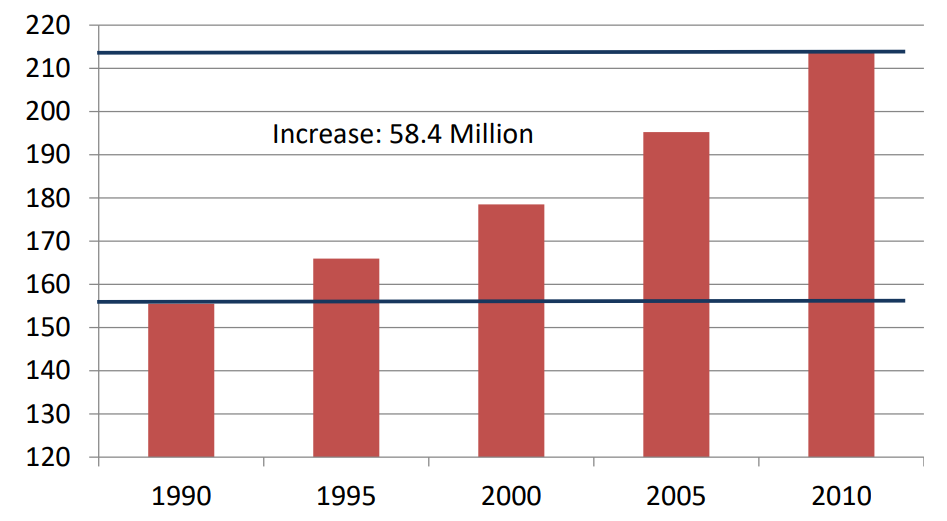
\includegraphics[width=4in]{images/ch11/1.png}
                \caption{Estimated number of international migrants in millions}
            \end{figure}
         \begin{itemize}
         \item There is a 58.4 million increase in the number of international migrants from 1990 to 2010, and this figure continues to increase.
         \end{itemize}
    \item Share of foreign-born population, selected countries
    \begin{figure}[H]
                \centering
                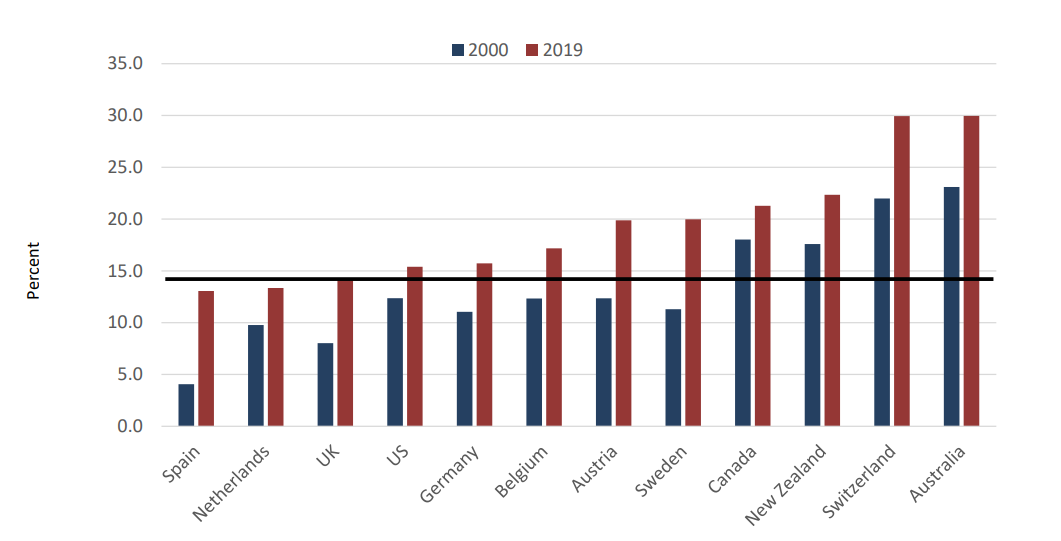
\includegraphics[width=4in]{images/ch11/2.png}
                \caption{Share of foreign-born population, selected countries}
            \end{figure}
         \begin{itemize}
         \item Blue bars indicate the shares of the foreign-born population in 2000, and red bars indicate the share of the foreign-born population in 2019. 
         \item The figure in Spain has tripled.
         \item In 2019, one in three people in Switzerland and Australia are foreign-born.
         \item The horizontal line is the 2019 average for the countries shown on the figure weighted be their total population.
         \end{itemize}
    \item Education of immigrants:
    \begin{figure}[H]
                \centering
                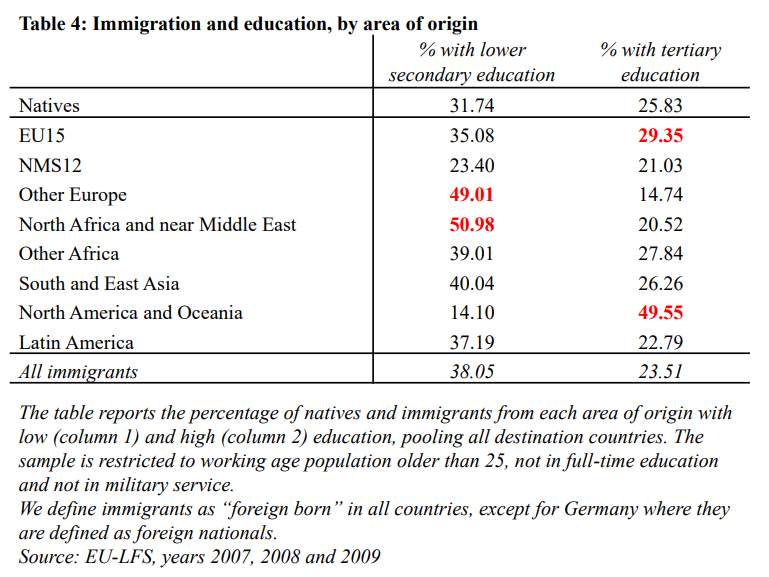
\includegraphics[width=4in]{images/ch11/6.png}
                \caption{Education of immigrants}
            \end{figure}
    \begin{itemize}
         \item The table reports the percentage of natives and immigrants from each area of origin with low (column 1) and high (column 2) education, pooling all destination countries. The sample is restricted to the working-age population older than 25, not in full-time education and not in military service. We define 
immigrants as “foreign born” in all countries, except for Germany where they are defined as foreign nationals.
         \item The share of immigrants with lower secondary education is high (around 50 percent) in Other Europe,  North Africa and near Middle East. The share of immigrants with tertiary education is high (around 50 percent) in North America and Oceania.
\end{itemize}
         
\end{itemize}


\subsection {Migration in the European context}
\begin{itemize}
\item Immigrants across Europe: Percentage and Origin
\begin{figure}[H]
                \centering
                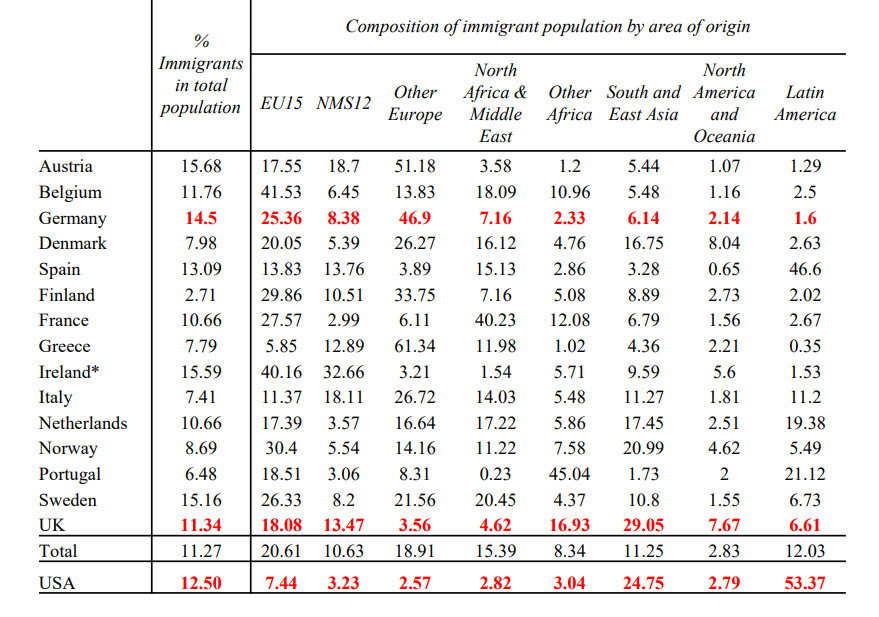
\includegraphics[width=4in]{images/ch11/3.png}
                \caption{Immigrants as a percentage of the total population, years 2007-2009}
            \end{figure}
            
\begin{itemize}
    \item There is a large difference in immigrant shares across different countries, and the composition by area is different.
\end{itemize}

\item Share of immigrants with tertiary education in selected EU countries, 2018
\begin{figure}[H]
                \centering
                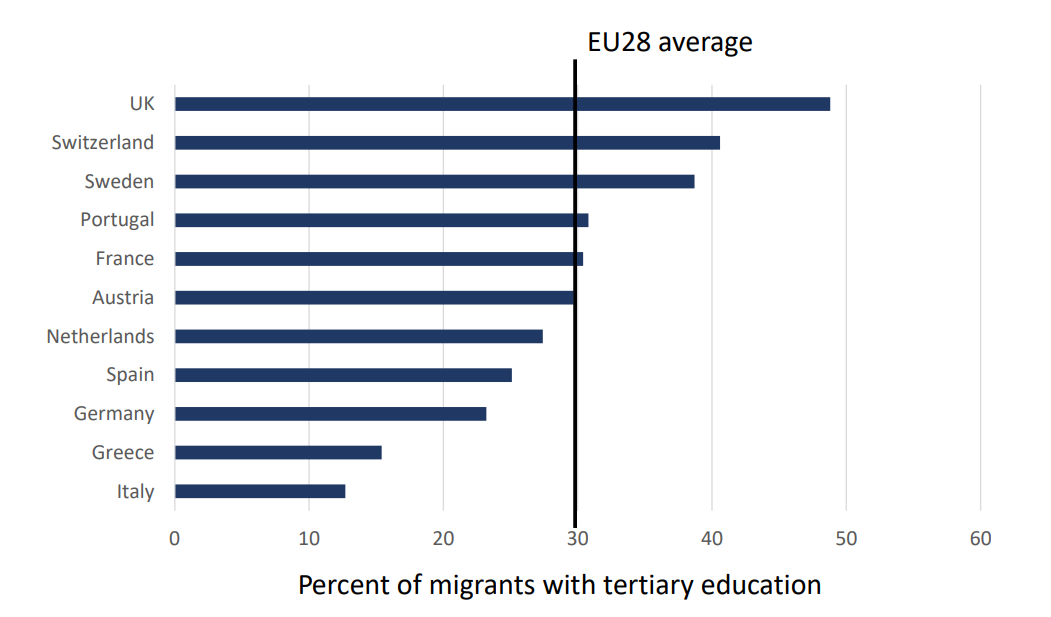
\includegraphics[width=4in]{images/ch11/4.png}
                \caption{Share of immigrants with tertiary education in selected EU countries, 2018}
            \end{figure}
            
\begin{itemize}
    \item Immigration is not a homogeneous phenomenon across countries. It is different in terms of education and origins across countries. 
    \item On average in EU28, one in three immigrants has tertiary education.
    \item The UK attracts the best-educated immigrants. Germany has a relatively low proportion of immigrants with tertiary education.
    \end{itemize}

\item Composition of Foreign-Born Population - Main Origin Countries, 2018
\begin{figure}[H]
                \centering
                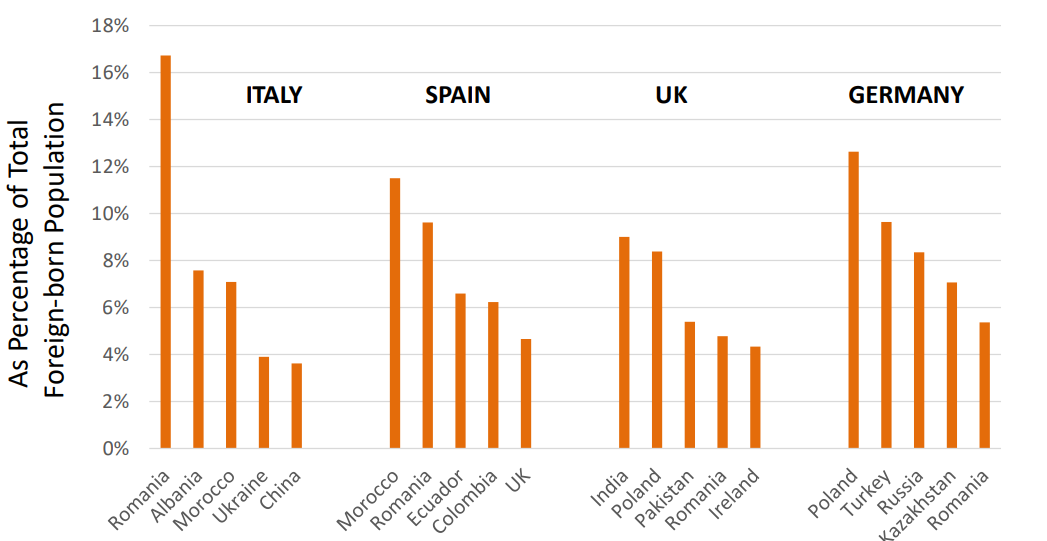
\includegraphics[width=4in]{images/ch11/5.png}
                \caption{Composition of Foreign-Born Population - Main Origin Countries, 2018}
            \end{figure}
\begin{itemize}
    \item There is little overlap in the main origin countries of immigrants across host countries.
\end{itemize}

\item Migration to Europe

\begin{itemize}
    \item Europe experienced \emphb{five major migration waves} after WW2.
    \item 1945 - 1960: Migrations caused by the war. About 20 million people displaced, mainly Germans.
    \item Second migration movement: economically motivated, started in the early 1950's - 1973 (labour migrations).
    \item Third wave of migration after 1973: family immigration and reunification of former labour migrants, and asylum migration.
    \item Fourth big movement: East-West migration, initiated in the late 1980's by a liberalisation of Soviet policy and accelerated by the fall of the Berlin wall in 1989.
    \item Early 1990’s: Movements as consequence of independence and democratisation, of wars inflicted on many areas within and around Europe.
    \item 2000’s: Globalisation, EU enlargement, and labour market rigidities let to
large immigration flows into, and across European countries.
    \item Question: Next decade? Immigration is likely to be increasingly fueled by war prosecution and inequality. Also, social media make people easier to get information about the host countries and then move.  Moreover, the large increase in population in Africa and, thus, the immigration imposes pressure on Europe and the US.
    \end{itemize}

\item Employment Differentials

\begin{itemize}
    \item We want to integrate and assimilate immigrants to realize their economic potential, as this is a win-win situation. When immigrants get higher wages in the host country, they pay more taxes.
    \item Immigrant-native employment differential
    \begin{figure}[H]
                \centering
                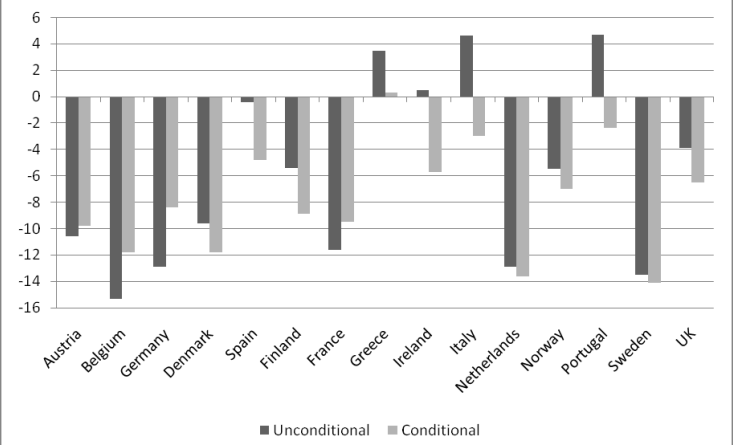
\includegraphics[width=4in]{images/ch11/7.png}
                \caption{Immigrant-native employment differential}
            \end{figure}
    \item Negative bars indicate that there is a higher employment probability of natives than immigrants. Positive bars indicate that there is a higher employment probability of immigrants than natives (e.g. Greece). Southern European countries tend to have positive bars unconditionally. Their shares of immigrants are small, but come only for joining the labour markets.
    \item Dark grey bars: unconditional; Light grey bars: conditional (on observed characteristics such as education, labour market experience).
\end{itemize}


\item Positions in National Earnings Distribution
\begin{figure}[H]
                \centering
                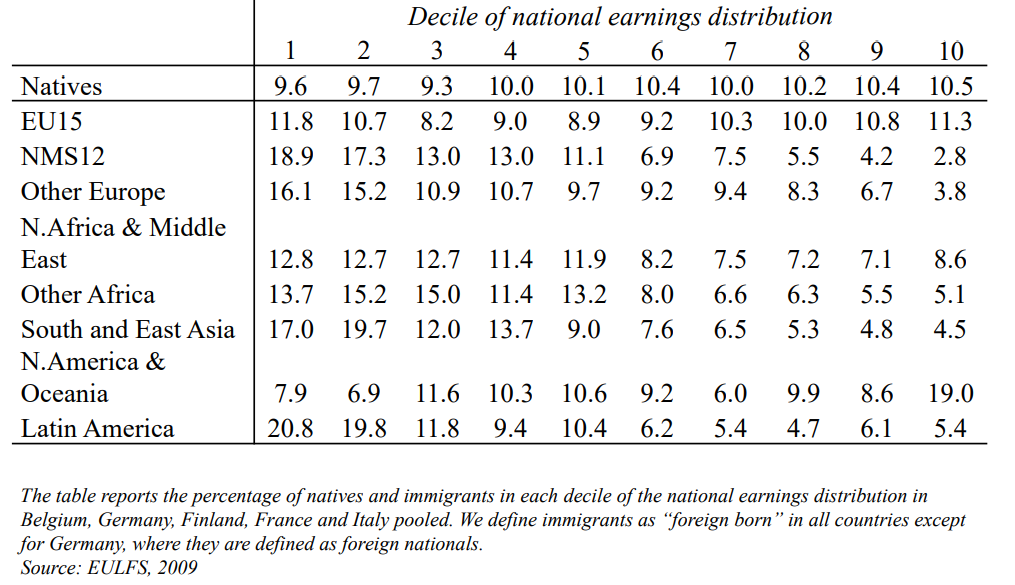
\includegraphics[width=4in]{images/ch11/8.png}
                \caption{Positions in National Earnings Distribution}
            \end{figure}
\begin{itemize}
    \item  The table reports \emphb{the percentage of natives and immigrants in each decile} of the national earnings distribution in Belgium, Germany, Finland, France and Italy pooled. We define immigrants as “foreign born” in all countries except for Germany, where they are defined as foreign nationals.
    \item EU15 and Oceania have a relatively larger share of immigrants in the top 10 percent decile of the earnings distribution, while other continents have relatively more immigrants in the lowest 10 percent decile. 
    \item Let's show the idea of this table in a graph below (only looking at EU and non-EU immigrants).
    \end{itemize}

\item Immigrant and native earnings distribution
\begin{figure}[H]
                \centering
                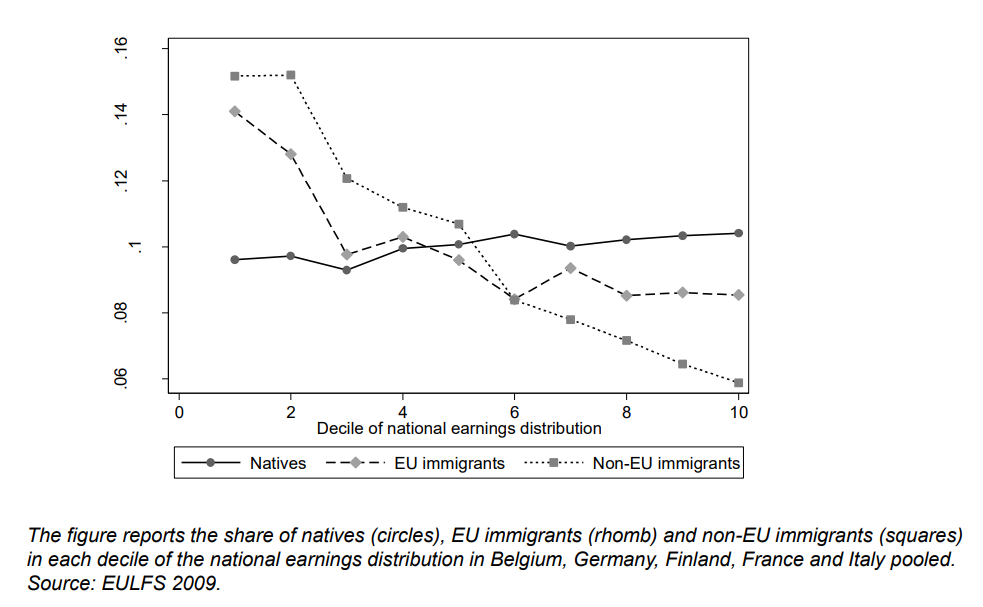
\includegraphics[width=4in]{images/ch11/9.png}
                \caption{Immigrant and native earnings distribution}
            \end{figure}
            
\begin{itemize}
    \item The figure reports \emphb{the share of natives (circles), EU immigrants (rhomb) and non-EU immigrants (squares) in each decile} of the national earnings distribution in Belgium, Germany, Finland, France and Italy pooled.
    \item We can see the natives' line is nearly a straight line. However,  EU immigrants and non-EU immigrants have a larger proportion in the lowest 10 percent decile of the earnings distribution (e.g. 15 percent of non-EU immigrants is in this decile), and they have a smaller proportion in the top 10 percent decile (e.g. only 6 percent of non-EU immigrants is in this decile). 
    \end{itemize}

\item Children of Immigrants
\begin{figure}[H]
                \centering
                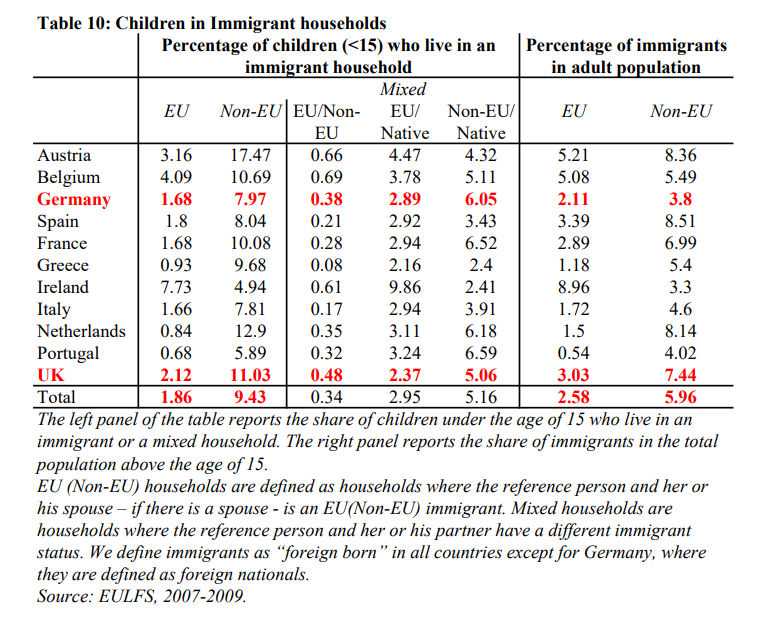
\includegraphics[width=4in]{images/ch11/10.png}
                \caption{Children of Immigrants}
            \end{figure}
            
\begin{itemize}
    \item The left panel of the table reports \emphb{the share of children under the age of 15 who live in an immigrant or a mixed household}. The right panel reports \emphb{the share of immigrants in the total population above the age of 15}. EU (Non-EU) households are defined as households where the reference person and her or his spouse – if there is a spouse - is an EU(Non-EU) immigrant. Mixed households are households where the reference person and her or his partner have a different immigrant status. We define immigrants as “foreign born” in all countries except for Germany, where they are defined as foreign nationals.
    \item 
    \end{itemize}

\item Poverty
\begin{figure}[H]
                \centering
                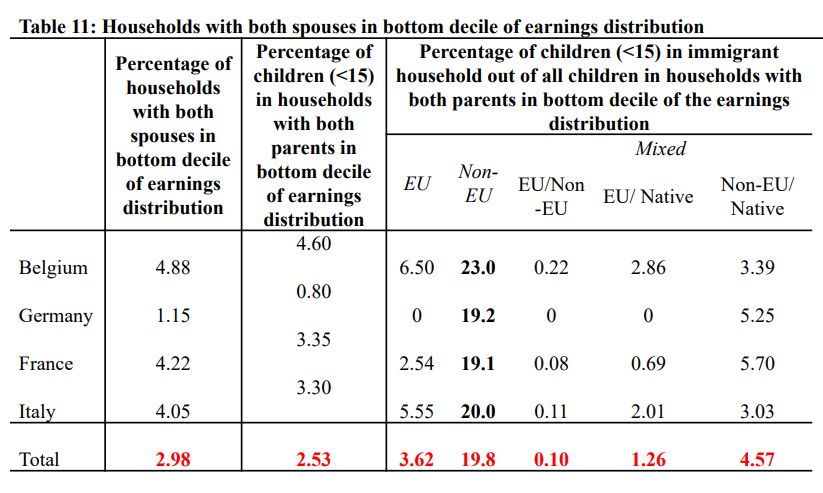
\includegraphics[width=4in]{images/ch11/11.png}
                \caption{Households with both spouses in the bottom decile of earnings distribution}
            \end{figure}
  \begin{itemize}
    \item The left panel shows the percentage of households with both spouses in the bottom decile of earnings distribution. The middle panel shows the percentage of children ($<$15) in households with both parents in the bottom decile of earnings distribution, which is quite in line with the left panel. The right panel shows \emphb{the percentage of children ($<$15) in immigrant households out of all children in households with both parents in the bottom decile of the earnings distribution}.      
    \item One in five (around 20 percent) of children ($<$15) in non-EU immigrant households live in poverty.
\end{itemize}

\end{itemize}
   
\section{The Migration Decision}
\begin{itemize}
    \item Two main reasons for migrations:
    \begin{itemize}
        \item Forced movement due to natural disaster or persecution
        \item Better economic prospects in other areas
    \end{itemize}
    \item This is still a distinction we draw today: between regulations for “asylum” immigrants and “economic” immigrants (1951 Geneva Refugee Convention). “Asylum” immigrants are not allowed to work in many countries, while economic immigrants can get access to the labour market.
    \item We will discuss here \emphb{economically motivated migrations}.
    \item Who is a Refugee? 1951 Geneva Convention for Refugees GCR:
    \begin{itemize}
        \item “[a person who] owing to a well-founded fear of being persecuted for reasons of race, religion, nationality, membership of a particular social group or political opinion, is outside the country of his nationality and is unable or, owing to such fear, is unwilling to avail himself of the protection of that country; …
        \item As of April 2015, 145 states have signed the 1951 Convention and 142 have signed both the Convention and the 1967 Protocol which endows the GCR with universal coverage. 
        \item Does not address civilians fleeing wars and conflicts (covered in different forms of temporary/subsidiary humanitarian protection)
    \end{itemize}
    \item Classification of Migrations
    \begin{figure}[H]
                \centering
                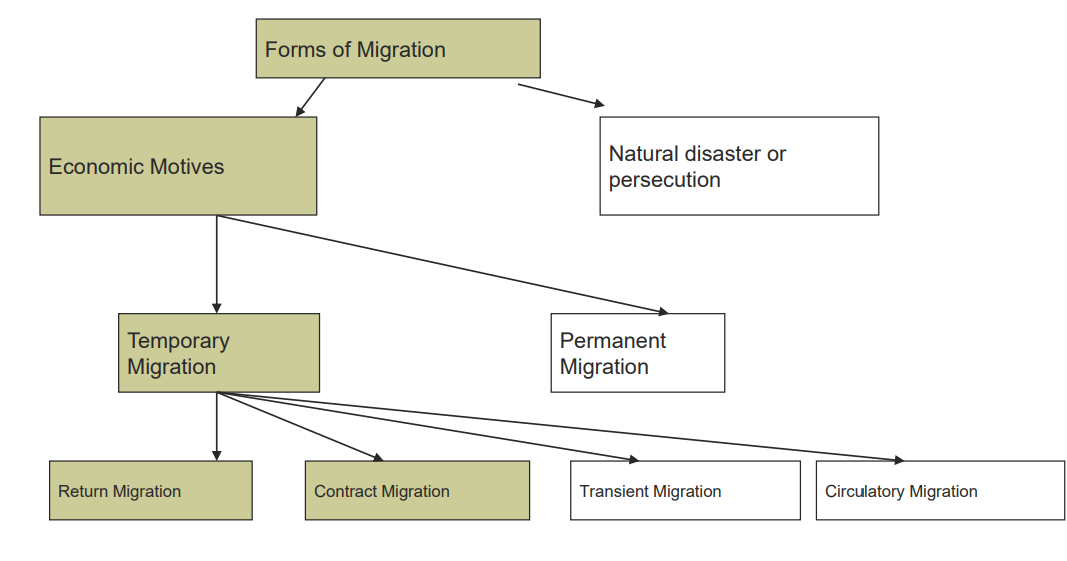
\includegraphics[width=4in]{images/ch11/12.png}
                \caption{Classification of Migrations}
            \end{figure}
    \item \empha{The Migration Decision Model}
    \begin{itemize}
        \item Migration decision of individual $i$ from O to D depends on the comparison of the discounted flow of future earnings in O and D, $y_{it}^O$ and $y_{it}^D$, net of migration cost $C_i$.
        $$ \sum_{t=0}^{T} y_{it}^D \frac{1}{{(1+r)}^t} - \sum_{t=0}^{T} y_{it}^O \frac{1}{{(1+r)}^t} - C_i = K_i $$

        \item Migration takes place whenever $K_i>0$
        \end{itemize}
    \end{itemize}

\section{Assimilation and performance of immigrants in the host countries}
\begin{itemize}
\item Empirical Literature: Immigrant Assimilation:

\begin{itemize}
\item Large literature in the economics of migration that is concerned with the estimation of immigrants’ earnings profiles.
\item First papers (e.g. Chiswick 1978): based on cross-section data (ignoring 
cohort effects) and assumed migrations to be permanent (ignoring selective out-migration).
\item Both assumptions are problematic, and we will discuss them in turn.
\end{itemize}

\item Log wage equations, for immigrants (I) and natives (N) :

$$(1)      lnw_i  ^I=b_0^I+b_1^IEX_i+b_2^IYSM_i+e_i^I$$

$$(2)      lnw_i  ^N=b_0^N+b_1^NEX_i+e_i^N$$

\begin{itemize}

\item $EX_i$: potential experience (computed as Age-years of schooling-6)
\item $YSM_i$: Years since migration
\item $b_1^I$: increase in earnings for each year of source country work experience for immigrants
\item $b_2^I$: additional increase in earnings each year spent in host country
\item $b_1^I+b_2^I$: earnings increase per year in the host country
\item $b_1^N$: earnings increase of natives per year of labour market experience
\item If $b_1^I+b_2^I > b_1^N$, earnings of immigrants grow faster in the host country than earnings of natives
\item $\delta=b_1^I+b_2^I-b_1^N$: rate of convergence of immigrant/native earnings. Measures degree of economic assimilation.
\end{itemize}

\item Economic Assimilation

\begin{figure}[H]
                \centering
                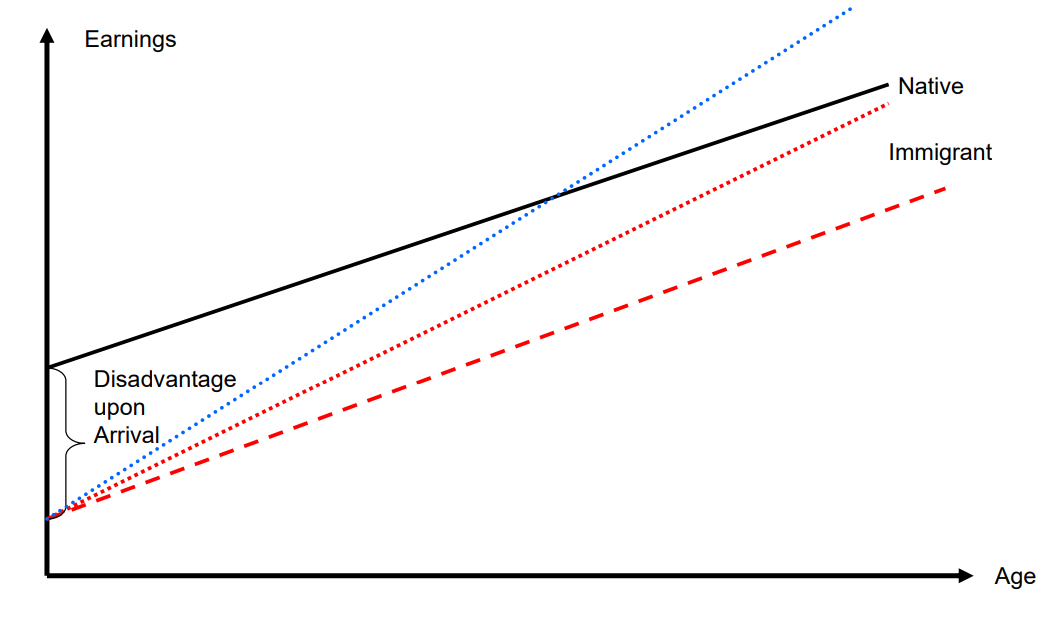
\includegraphics[width=4in]{images/ch11/13.png}
                \caption{Economic Assimilation}
            \end{figure}

\item Immigration and Assimilation
\begin{itemize}
\item Chiswick (1978): uses 1970 US census data to estimate
a regression similar to the one above.
\item Main Findings:
\begin{itemize}
\item Immigrants have upon arrival an earnings disadvantage of about 17 percent
\item After about 10-15 years in the US labour market, earnings of immigrants overtake those of native workers.
\end{itemize}
\item He explains this finding with immigrants having “more innate  ability, is more highly motivated towards labour market success, or self-finance larger investments in post-school training”.
\end{itemize}

\end{itemize}

\section{Challenges to the estimation of immigrants' assimilation profiles}

\subsection{Cohort Effects}
\begin{itemize}
\item Borjas (1985): estimation based on cross-sectional data may lead to misleading conclusions, because immigrants who differ in their years of residence in the host country have also arrived at different points in time.
\item If entry wages of immigrants change over time, then this may be picked up by the coefficient on the years since migration variable, confounding differences in immigrant cohort quality with assimilation.
\end{itemize}
    \begin{figure}[H]
                \centering
                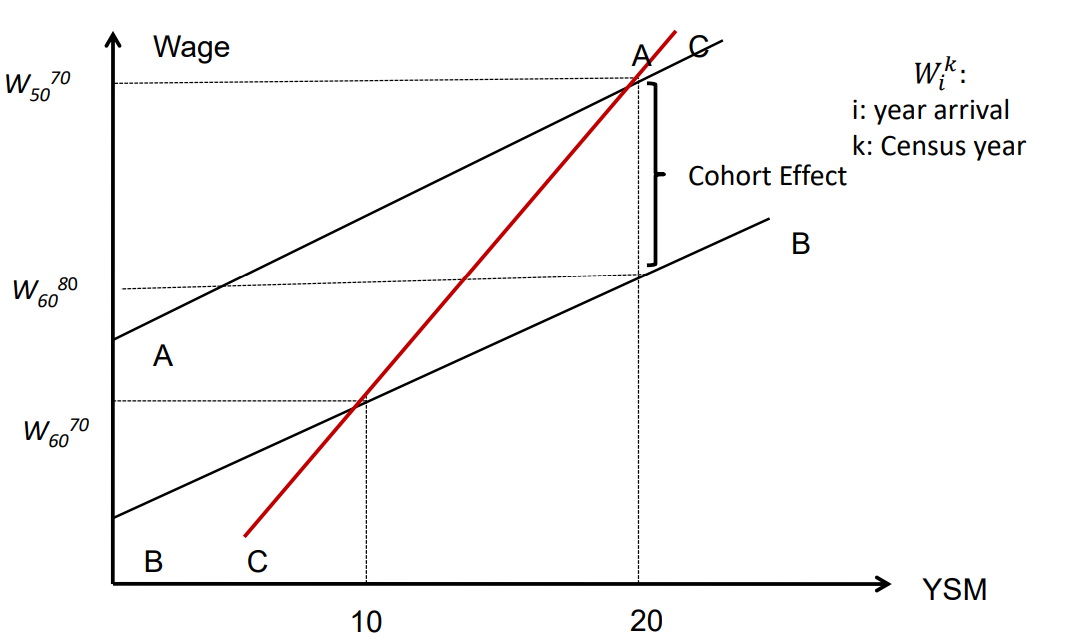
\includegraphics[width=4in]{images/ch11/14.png}
                \caption{Immigration and Assimilation: Cohort Effects}
            \end{figure}
\begin{itemize}            
\item 1970 census: measures wages   $w_{50}^{70}$ for those with 20 years of residence, and $w_{60}^{70}$ for those with 10 years of residence.
\item Wage growth in host country: $\frac{\Delta w}{\Delta YSM}$; this is slope of line CC.
\item Overestimate of immigrant wage growth if negative cohort effects.
\item Identification problem, can be solved through additional information (or assumption, as Chiswick has done, by assuming there are no cohort effects)
\item Use further census year and observe the same cohort of immigrants at two different points in time. If that additional information comes in form of the 1980 census, the cross-sectional estimate decomposes as
$$\frac{w_{50}^{70}-w_{60}^{70}}{10}=\frac{w_{60}^{80}-w_{60}^{70}}{10}-\frac{w_{50}^{70}-w_{60}^{80}}{10} $$

where the first term is equal to the wage growth of cohort 60, while the second term is equal to the cohort effect.
\item Lower initial wages of subsequent cohorts may lead to an overestimate of cross-sectional wage profiles, while improvement in cohort quality leads to an underestimate.
\end{itemize}

\subsection{Selective outmigration}